\chapter{Технологический раздел}
\label{cha:impl}

\section{Выбор языка программирования}
В настоящей работе для реализации проекта был выбран язык программирования C++ по следующим причинам:
\begin{itemize}
 \item является языком высокого уровня, что позволяет разрабатывать программное обеспечение на высоком уровне абстракций,
 \item обладает преимуществами разработки программного обеспечения при использовании объектно-ориентированного подхода, обеспечивает 
 свойства объектно-ориентированного подхода: инкапсуляцию, наследование, полиморфизм,
 \item предоставляет удобные средства для обработки исключительных ситуаций,
 \item обладает набором стандартных коллекций (вектор, список, и другие),
 \item является кроссплатформенным.
\end{itemize}

Для разработки и отладки приложения была выбрана среда разработки Visual Studio 2010. 
Эта среда разработки обладает удобным и интуитивно понятным интерфейсом 
пользователя, удобными средствами разработки и отладки приложений, 
а так же встроенными средствами для разработки GUI.

\section{Использование сторонних библиотек}
В разрабатываемом проекте необходимо производить обработку видео, выбранных пользователем. 
Так как существует большое количество форматов представления графических данных, для сокращения 
времени разработки использовалась библиотека OpenCV, которая предоставляет интерфейс для чтения 
и записи графических данных в файлы основных используемых форматов. Библиотека OpenCV является 
свободно распространяемой, имеет обширную документацию, постоянно обновляется, 
что является ее преимуществами перед другими библиотеками.
Для работы прямого и обратного вейвлет-преобразований важна скорость работы. 
Так как вейвлет-преобразование состоит в умножении строк матрицы графических данных 
на матрицу преобразования, эту операцию можно распределить по потокам. 
Для распределения операций по потокам использовался открытый стандарт для распараллеливания программ на 
языке C++ OpenMP. Наличие инструментов 
OpenMP в среде разработки Visual Studio 2010 также упрощает ее использование.  
Стандарт OpenMP является свободно распространяемым, имеет обширную документацию, 
постоянно обновляется, что является его преимуществами перед другими аналогичными инструментами.

\section{Требования к программной совместимости}
Разработка и тестирование программного обеспечения веласть на компьютере с установленной операционной системой Windows 7.
Для корректной работы исполняемого файла необходимо наличие библиотек OpenCV в одной директории с исполняемым файлом.
Минимальные Требования к компьютеру для запуска разработанного программного обеспечения указаны в таблице \ref{tab:comp}.

\begin{table}[ht]
  \caption{Минимальные требования к техническим характеристикам компьютера}
  \begin{tabular}{|p{5cm}|p{10cm}|}
  \hline
  Характеристика      & Требуемое значение \\
  \hline
  Процессор  &  Intel Core 2 Duo CPU T5800 2.00GHz x2\\
  \hline
  Оперативная память       & 2 Гб \\
  \hline
  Операционная система  & Windows 7 x32 \\
  \hline
  Жесткий диск  & 1Гб свободного дискового пространства \\
  \hline
  \end{tabular}
  \label{tab:comp}
\end{table}

\section{Разработанные классы в программном комплексе}
В соответствии со схемой модулей \ref{fig:modules} была разработана структура классов, изображенная на рисунке \ref{fig:classes}.

\begin{figure}
  \centering
  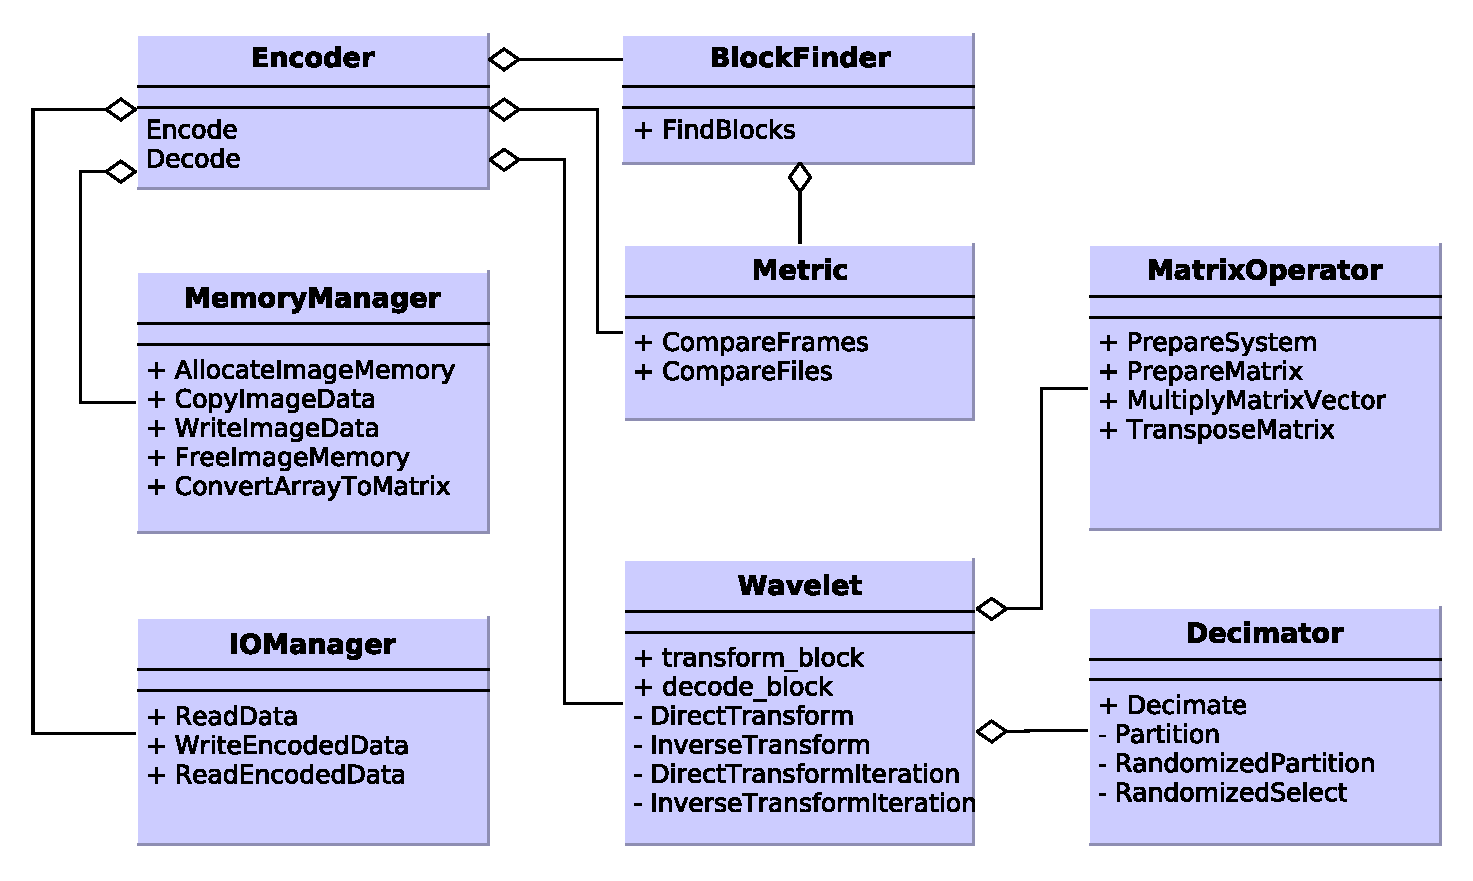
\includegraphics[scale=0.6]{inc/graphics/classes.pdf}
  \caption{Диаграмма классов разрабатываемой системы}
  \label{fig:classes}
\end{figure}

Класс \texttt{Encoder} является точкой входа в разрабатываемую систему. 
Содержит методы:
\begin{itemize}
 \item \texttt{void Encode(char *fileName, int rate);}
 \item \texttt{void Decode(char *fileName);}
\end{itemize}
 
В метод \texttt{Encode} передаются имя входного файла 
с графическими данными
и коэффициент децимации. Метод выполняет анализ графических дынных, применяет вейвлетное преобразование к графическим данным, 
проводит децимацию и кодирование коэффициентов, осуществляет запись кодированных коэффициентов в файл.
В метод \texttt{Decode} передается имя входного файла с закидированными данными. Метод проводит чтение закодированных коэффициентов 
из файла, применяет обратное вейвлетное преобразование, составляет из преобразованых блоков кадры и проводит воспроизведение последовательности кадров.

Класс \texttt{Wavelet} вейвлетных преобразований получает на вход графические данные и параметры преобразования, 
применяет к данным указанное преобразование, возвращает преобразованные данные. Содержит следующие методы:

\begin{itemize}
 \item \texttt{std::vector<int> transform\_block(IplImage **block, int block\_size, int nChannels, int height, int width, int system, int savePerc)} - 
 метод прямого вейвлетного преобразования. Параметры: графические данные \texttt{block}, размер блока \texttt{block\_size}, 
 количество каналов \texttt{nChannels}, ширина \texttt{width} кадра, 
высота \texttt{height} кадра, система коэффициентов преобразования \texttt{system}
 \item \texttt{IplImage ** decode\_block(std::vector<int> out\_data, int block\_size, int nChannels, int height, int width, int system)} - 
 функция выполнения обратного вейвлет-преобразования.
 Параметры: графические данные \texttt{out\_data}, размер блока \texttt{block\_size}, количество каналов \texttt{nChannels}, ширина \texttt{img\_width} кадра, 
 высота \texttt{img\_height} кадра, система коэффициентов преобразования \texttt{system}.
 \item \texttt{void DirectTransform(float ****image\_data, int nChannels, int img\_width, int img\_height, int img\_depth, 
 int width, int height, int depth, int transform\_type);} 
 - метод прямого вейвлетного преобразования блока. Параметры:
 графические данные блока \texttt{image\_data}, количество каналов \texttt{nChannels}, ширина \texttt{img\_width} блока, 
высота \texttt{img\_height} блока, глубина \texttt{img\_depth} блока, ширина \texttt{width} рассматриваемой области, 
высота \texttt{height} рассматриваемой области, глубина \texttt{depth} рассматриваемой области, система коэффициентов преобразования \texttt{transform\_type},
 \item \texttt{void InverseTransform(float ****image\_data, int nChannels, int img\_width, int img\_height, int img\_depth, 
 int width, int height, int depth, int transform\_type);} - 
 - метод обратного вейвлетного преобразования блока. Параметры:
 графические данные блока \texttt{image\_data}, количество каналов \texttt{nChannels}, ширина \texttt{img\_width} блока, 
высота \texttt{img\_height} блока, глубина \texttt{img\_depth} блока, ширина \texttt{width} рассматриваемой области, 
высота \texttt{height} рассматриваемой области, глубина \texttt{depth} рассматриваемой области, система коэффициентов преобразования \texttt{transform\_type},
 \item \texttt{void DirectTransformIteration(float ****image\_data, 
 int channel\_index, int part\_count, int index1, int index2, 
 int direction, const std::vector<std::vector<float> > \&matrix\_ad);} – метод выполнения итерации прямого вейвлет-преобразования. 
 Параметры: графические данные \texttt{image\_data}, номер канала \texttt{channel\_index}, 
 длина вектора для преобразования \texttt{part\_count}, номера векторов для преобразования в двух измерениях \texttt{index1} и \texttt{index2}, 
 направление \texttt{direction}, матрица преобразования \texttt{matrix\_ad}  
 \item \texttt{void InverseTransformIteration(float ****image\_data, 
 int channel\_index, int part\_count, int index1, int index2, int direction, 
 const std::vector<std::vector<float> > \&matrix\_ad);} – функция выполнения итерации обратного вейвлет-преобразования.
 Параметры: графические данные \texttt{image\_data}, номер канала \texttt{channel\_index}, 
 длина вектора для преобразования \texttt{part\_count}, номера векторов для преобразования в двух измерениях \texttt{index1} и \texttt{index2}, 
 направление \texttt{direction}, матрица преобразования \texttt{matrix\_ad}.
\end{itemize}

Метод \texttt{transform\_block} был разработан в соответствии со схемой прямого вейвлетного преобразования, представленной на рисунке \ref{fig:figalgdir}.
Код метода представлен в литинге \ref{lst:direct}. Метод \texttt{decode\_block} выполняет схожие действия в обратном порядке.

\begin{lstlisting}[style=realcode,caption={Код метода transform\_block},label=lst:direct]
std::vector<int> transform_block(IplImage **block, int block_size, int nChannels, int height, int width, int system, int savePerc){
  float ****block_data = new float***[block_size];
  for (int i = 0; i < block_size; ++i){
    float ***image_data = NULL;
    image_data = AllocateImageMemory(nChannels, height, width, image_data);
    auto frame = block[i];
    CopyImageData(frame, image_data, nChannels, height, width);
    block_data[i] = image_data;
  }

  DirectTransform(block_data, nChannels, width, height, block_size, width, height, block_size, system);
  std::vector<int> out_data = Decimate(block_data, nChannels, width, height, block_size, savePerc);
  for (int i = 0; i < block_size; ++i)
    FreeImageMemory(nChannels, height, width, block_data[i]);
  delete[] block_data;
  return out_data;
}
\end{lstlisting}

Класс \texttt{BlockFinder} содержит метод поиска блоков на последовательности кадров:
\texttt{IplImage ** FindBlocks(IplImage *frames, int framesSize);}, где \texttt{frames} - последовательность кадров, \texttt{framesSize} - длина последовательности кадров.

Класс \texttt{Metrix} служит для поиска границ блоков,
а так же для оценки качества видео после применения алгоритмов кодирования. Содержит методы поиска разности между кадрами и между последовательностями кадров:
\begin{itemize}
 \item \texttt{float CompareFrames(IplImage \&frame1, IplImage \&frame2);}, где \texttt{frame1} и \texttt{frame2} - сравниваемые кадры,
 \item \texttt{float CompareFiles(IplImage *frames1, IplImage *frames2);}, где \texttt{frames1} и \texttt{frames2} - сравниваемые файлы.
\end{itemize}

Класс \texttt{MatrixOperator} производит умножение матрицы на вектор, а так же составление матриц для указанного вейвлет-преобразования. Содержит следующие методы:
\begin{itemize}
 \item \texttt{void PrepareMatrix(std::vector<std::vector<double> > \&matrix, int dimension, const std::vector<double> \&system)} - 
 функция составления матрицы преобразования указанной размерности для указанной системы коэффициентов
 Параметры: матрица преобразования \texttt{matrix}, размерность матрицы, \texttt{dimension}, система коэффициентов system.

 \item \texttt{std::vector<double> PrepareSystem(int transform\_type)} - функция получения набора коэффициентов указанной системы коэффициентов
 Параметры: тип преобразования \texttt{transform\_type}.

 \item \texttt{void MultiplyMatrixVector(const std::vector<std::vector<double> > \&matrix, double ***image\_data, int channel\_index, 
 int part\_count, int vector\_index, int direction)} - функция умножения матрицы на вектор графических данных
 Параметры: матрица преобразования \texttt{matrix}, графические данные \texttt{image\_data}, 
 номер канала \texttt{channel\_index}, длина вектора для преобразования \texttt{part\_count}, 
 номер вектора для преобразования \texttt{vector\_index}, направление (строка или столбец) \texttt{direction}.

 \item \texttt{void TransposeMatrix(std::vector<std::vector<double> > \&matrix)} - функция транспонирования матрицы
 Параметры: матрица преобразования \texttt{matrix}.

\end{itemize}

Класс \texttt{Decimator} выбора значимых получает от управляющего модуля графические данные 
и степень сжатия, удаляет указанную часть данных, возвращает обработанные данные. Содержит методы:
\begin{itemize}
 \item \texttt{std::vector<int> Decimate(float ****image\_data, int nChannels, int width, 
 int height, int depth, char decimatio\_ratio);} – функция удаления части графических данных. 
Параметры: графические данные \texttt{image\_data}, количество каналов \texttt{nChannels}, 
ширина \texttt{width}, высота \texttt{height}, глубина \texttt{depth} блока, процент сохраняемых данных \texttt{decimation\_ratio}.
\item \texttt{float RandomizedSelect(std::vector<float> \&numbers, int left, int right, int level)} - метод поиска порядковой статистики, где 
\texttt{numbers} - рассматриваемый набор данных, \texttt{left} - левая граница части массива для поиска, \texttt{right} –
правая граница части массива для поиска, \texttt{level} – номер искомой порядковой
статистики,
\item \texttt{int Partition(std::vector<float> \&numbers, int left, int right);} - 
метод выбора опорного элемента случайным образом. Параметры:
\texttt{numbers} - рассматриваемый набор данных, \texttt{left} - левая граница части массива для поиска, \texttt{right} –
правая граница части массива для поиска,
\item \texttt{int RandomizedPartition(std::vector<float> \&numbers, int left, int right);} - метод выбора опорного элемента. Параметры:
\texttt{numbers} - рассматриваемый набор данных, \texttt{left} - левая граница части массива для поиска, \texttt{right} –
правая граница части массива для поискаю
\end{itemize}

Класс \texttt{IOManager} производит чтение и запись в файл закодированных графических данных. Содержит методы:

\begin{itemize}
 \item \texttt{void ReadData(char file\_name[])} – функция чтения графических данных из файла.
 Параметры: имя файла \texttt{file\_name}.
 \item \texttt{void WriteEncodedData(char file\_name[], std::vector<int> data)} – функция записи кодированных данных в файл. 
 Параметры: имя файла \texttt{file\_name}, данные \texttt{data}.
 \item \texttt{std::vector<int> ReadEncodedData(char file\_name[])} – функция чтения кодированных данных из файла. Параметры: имя файла \texttt{file\_name}.
\end{itemize}

Формат файла с закодированными данными представлен на рисунке \ref{fig:format}, где NChannels - количество каналов для представления цвета, Width - ширина кадра,
Heigth - высота кадра, BlockLength - длина очередного блока, BlockData - графические данные очередного блока.

\begin{figure}
  \centering
% [width=0.5\textwidth] --- регулировка ширины картинки
  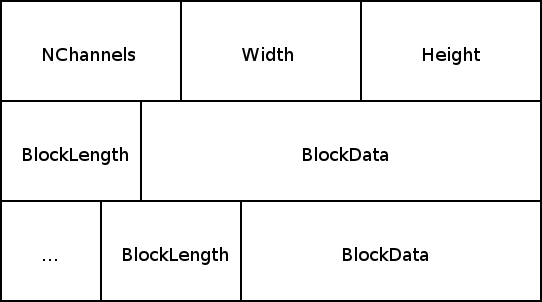
\includegraphics[scale=0.5]{inc/graphics/format.png}
  \caption{Формат файла с закодированными графическими данными}
  \label{fig:format}
\end{figure}

Класс \texttt{MemoryManager} предназначен для управления памятью для графических данных. Содержит методы:
\begin{itemize}
 \item \texttt{double*** AllocateImageMemory(int channels\_count, int row\_count, int column\_count, double ***image\_data)} – 
 функция выделения памяти для данных о кадре Параметры: количество каналов \texttt{channels\_count}, 
 количество строк \texttt{row\_count}, количество столбцов \texttt{column\_count}, данные о кадре \texttt{image\_data}.
 \item \texttt{void FreeImageMemory(int channels\_count, int row\_count, int column\_count, double ***image\_data)} – 
 функция освобождения памяти для данных о кадре
 Параметры: количество каналов \texttt{channels\_count}, количество строк \texttt{row\_count}, 
 количество столбцов \texttt{column\_count}, данные о кадре \texttt{image\_data}.
 \item \texttt{void CopyImageData(IplImage *in\_image, double ***image\_data)} – функция копирования графических данных из кадра во внутреннюю структуру данных
 Параметры: входной кадр \texttt{in\_image},  данные о кадре \texttt{image\_data}.
 \item \texttt{void WriteImageData(double ***image\_data, IplImage *in\_image)} – функция копирования графических данных из внутренней структуры данных в кадр.
 Параметры: кадр \texttt{in\_image},  данные о кадре \texttt{image\_data}.
 \item \texttt{void ConvertArrayToMatrix(std::vector<int> \&data, double ***image\_data)} – функция преобразования считанного 
 кодированного массива в матрицу графических данных кадра
 Параметры: массив данных \texttt{data},  данные о кадре \texttt{image\_data}.
\end{itemize}

\section{Кадры, получаемые при применении вейвлетного преобразования}
Пример кадра из видео, к которому было применено вейвлетное преобразование, представлен в приложении \ref{app:ex}.
Вейвлет-преобразование выполнено с сохранением 10\% (вверху справа), 5\% (внизу слева), 2\% (внизу справа) коэффициентов. 
Вверху слева представлено исходное изображение. На представленном изображении видно, что при сохранении большего количества коэффициентов
наблюдается эффект сглаживания однородных областей. При уменьшении количества сохраненяемых коэффициентов на изображении наблюдается появление 
артефактов. Мелкие детали, представленные на исходном изображении, при высокой степени сжатия размываются, образуя пятна на получаемом изображении.

\section{Пользовательский интерфейс разрабатываемого программного комплекса}
Пользовательский интерфейс разрабатываемого программного комплекса представлен на рисунке \ref{fig:ui}.
В соответствии с разработанными сценариями функционирования программного комплекса был спроектирован пользовательских интерфейс.

Предоставлена возможность выбора исходного файла с графическими данными. При нажатии на кнопку выбора файла пользователю предлагается 
стандартный диалог выбора файла, принятый в разрабатываемой операционной системе. После выбор файла имя выбранного файла отображается в 
текстовом поле. 

Ползователю предоставляется возможность указать процент сохраняемых данных в текстовом поле. Введенное число должно быть целым в диапазоне от 1 до 99.

При нажатии на кнопку <<Кодировать>> выполняется поиск блоков, прямое вейвлетное преобразование блоков, децимация графических данных и запись закодированных данных в файл.
При нажатии на кнопку <<Декодировать>> выполняется чтение из файла, обратное вейвлетное преобразование, воспроизведение графических данных.

При отсутствии выбранного файла или при ошибочном вводе процента сохраняемых данных отображается сообщение об ошибке.

\begin{figure}
  \centering
% [width=0.5\textwidth] --- регулировка ширины картинки
  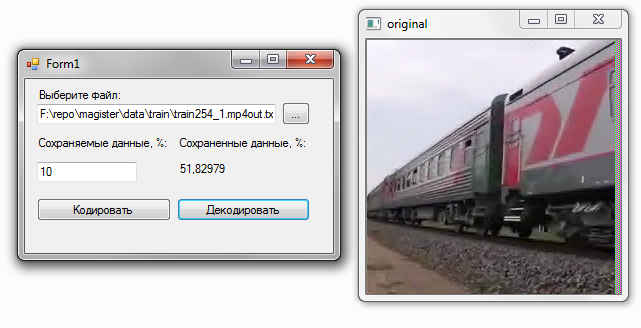
\includegraphics[scale=0.75]{inc/graphics/ui.png}
  \caption{Пользовательский интерфейс разрабатываемого программного комплекса}
  \label{fig:ui}
\end{figure}
